\chapter{Paraview}

ICE features functionality for visualizing models using ParaView.

\section{Installation and Configuration}

ParaView use for ICE requires a Mac OS or Linux operating system, as ICE does
not currently support ParaView connections to Windows hosts. However, it will
still be possible to connect from ICE on Windows to a Mac or Linux machine
that has ParaView installed. You will also need an installation of ParaView on
your local machine.
ParaView can be downloaded from its \href{http://www.paraview.org/download/}{official website}. The ICE
development team recommends using the latest available version of ParaView,
currently 5.0 at the time of this writing. You will further need a custom
Python HTTP web server implementation, which can be downloaded from the
\href{http://eclipseice.ornl.gov/downloads/paraview/scripts/http_pvw_server.py}{Oak
Ridge website}.

\subsection{Configuring the ParaView Connection}

Once ParaView is running, ICE must be configured to connect to the server. This
is done through specifying a default connection in the ICE Preferences page.
This process only needs to be performed once. After initially creating the
connection, ICE will attempt to connect to ParaView on that port each time it is
launched.

To set the connection, select Window $\rightarrow$ Preferences\ldots in ICE's
menu bar. (On Mac OS X, Preferences\ldots is located under ICE instead of
Windows.) Select Visualization $\rightarrow$ ParaView in the tree on the left
side of the Preferences window.

\begin{center}
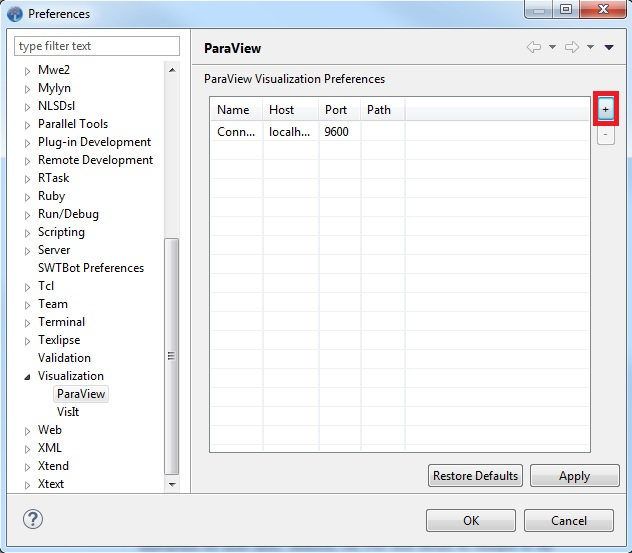
\includegraphics[width=12cm]{images/paraviewpreferencepage_ice}
\end{center}

Press the button with a ''+" symbol in the upper right (highlighted in the image
above) to add a new row to the table. Click on cells in the new row to edit
their values. 

\textbf{Name:} The connection's name. The default value will be fine.

\textbf{Host:} The hostname for the machine that will run ParaView. Use "localhost" if the machine running ICE will also be used to run ParaView.

\textbf{Port:} The port number on which the ParaView server will run. The default value will be fine, but if you change it, it must different from the Visualizer Port.

\textbf{Path:} The path to your ParaView installation. 

On Linux, the path will end with the top level folder into which ParaView was unzipped. For example, if you have a folder named ParaView on your desktop that contains the bin, doc, lib, and share folders, then your path would be /home/username/Desktop/ParaView. 

On Mac, the path will end with the folder containing your ParaView.app. For example, if you have installed ParaView to your Applications folder, the path will simply be /Applications

\textbf{Server Script Path:} The full path to the http\_pvw\_server.py file,
ending with the folder containing it. For example if the file is on your desktop, the path might be /home/username/Desktop.

\textbf{Visualizer Port:} The port number for the ParaView web visualizer. The default value will be fine, but if you change it, then it must be different from the port number you provide for Port.

\textbf{Remote OS:} The operating system of the remote machine on which ParaView will be launched. If you want to launch ParaView on your local machine, ignore this cell. Otherwise, specify either "Linux" or "OSx".

\textbf{Remote ParaView Version Number:} The version of ParaView you are using. This may be ignored unless you are launching a remote ParaView session on a Linux machine. You can check your installation's version number by looking inside the top level \textbf{lib} folder. It will contain a folder named paraview- followed by the version number.

Once finished editing the cells in the new row, press Apply, then OK. ICE will
then launch the ParaView server and connect to it. If you are connecting to a remote machine, you will be prompted for permission to make the remote connection and asked for a password.

\section{Opening a ParaView File} 

To open a ParaView Plot Editor, a file that uses this editor must first be
placed in the Project Explorer. This view lists files imported into ICE. To
access the Project Explorer, use the the menu bar at the top of the window and
navigate to Window $\rightarrow$ Show View $\rightarrow$ Project Explorer.
Depending on the active Eclipse perspective, opening this view may require
selecting Other\ldots and finding the Project Explorer in the dialog under the
General category in the tree.

By default, the Project Explorer should automatically import the
ICEFiles/default and ICEFiles/itemDB folders. If it does not, or if you want to
import a different folder into ICE, right click in the Project Explorer and
select Import\ldots from the context menu. Then, select General $\rightarrow$
File System from the tree, and press the Next button. Select directories and/or
files to import into the Project Explorer, and enter which folder they should
be imported into, as shown below.

\begin{center}
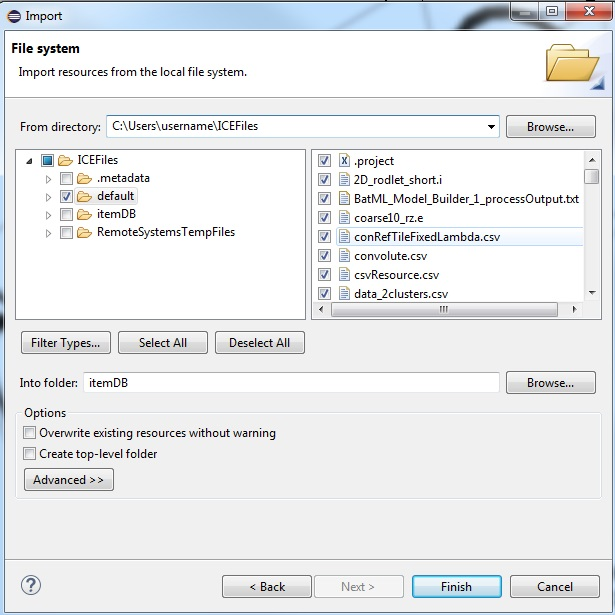
\includegraphics[width=12cm]{images/ImportFileDialog}
\end{center}

Once a file is in the Project Explorer, simply double click on it to open it in
ParaView. Local ParaView connections can only open local files, while remote ParaView connections can only open files on the remote host.

\subsection{Using ParaView}

\subsubsection{Camera Controls}

The Plot Editor allows the user to rotate the model by clicking and dragging
inside the display area or adjust the zoom by scrolling the mouse wheel.

\begin{center}
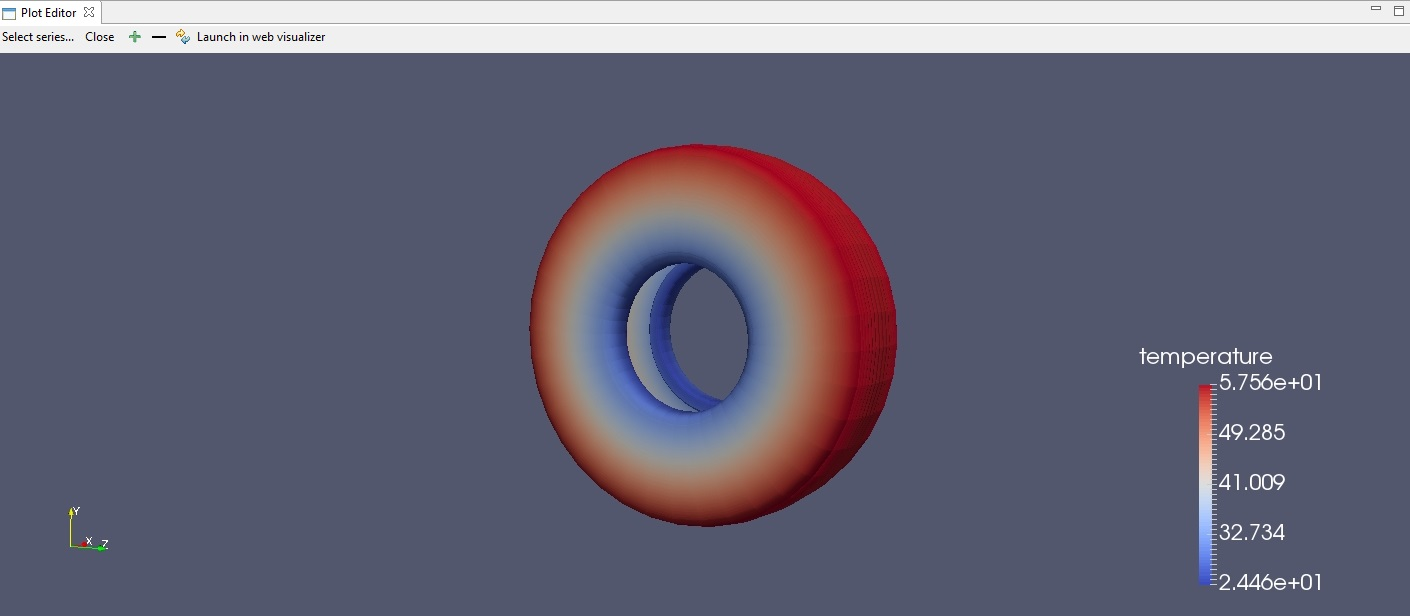
\includegraphics[width=12cm]{images/ParaViewPlotEditor}
\end{center}

The buttons in the upper left can also be used to manipulate the camera. The
green plus sign will zoom in, while the black minus sign will zoom out. The
yellow and blue circular arrow button will reset the camera to its default
position.

\subsubsection{Selecting the Plot}

Pressing the Select Series\ldots button will open a dialog which lists the
various plots in the opened file. Simply select one and click OK to open it. 

\begin{center}
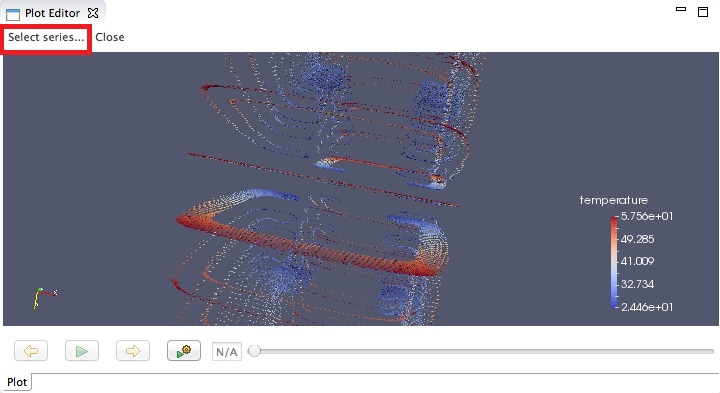
\includegraphics[width=12cm]{images/ParaViewPlotEditorSelectSeriesButton}
\end{center}

\subsubsection{Setting the Plot Representation} 

ParaView is capable of displaying plots in several different representations,
such as points or surfaces. To switch between plot type, right click inside the Plot
Editor's display area and select one of the listed options under the
Representation category in the context menu.

\begin{center}
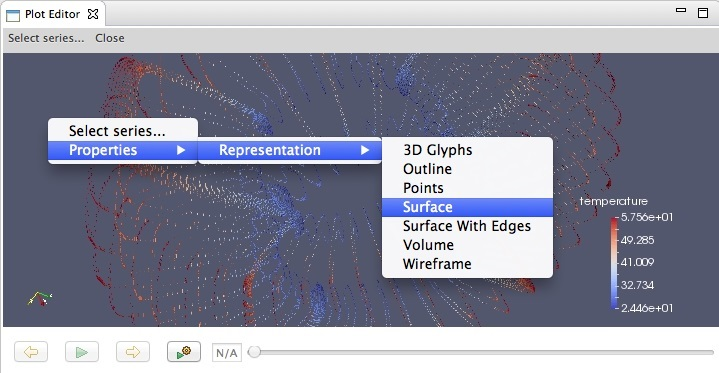
\includegraphics[width=12cm]{images/ParaViewRepresentationDropDown}
\end{center}

\subsubsection{Animation and Time Data}

The Plot Editor features a time slider widget at the bottom of the screen. 

\begin{center}

\includegraphics[width=12cm]{images/TimeSliderWidget}
\end{center}

The controls, in order of left to right, are:

1) Return to the previous time step.

2) Automatically play the plot as an animation by displaying the time steps
sequentially. 

3) Advance to the next time step. 

4) Opens an options menu that allows the user to set the playback speed, toggle
whether the animation should loop when it reaches the end, and set the plot to
the first or last time step.

5) A display for the current time step. It can be edited to set the plot to an
arbitrary time step. 

6) A slider that shows the current time step's position on the timeline. The
slider can be dragged around the timeline, setting the plot's time step
accordingly.

\section{Accessing a ParaView Web Server}

It is also possible to access the full ParaView web viewer application inside of
ICE. This allows for full access to all the web viewer's features.

\subsection{Accessing the Visualizer}

First, you must open a Plot Editor as described above.

\begin{center}
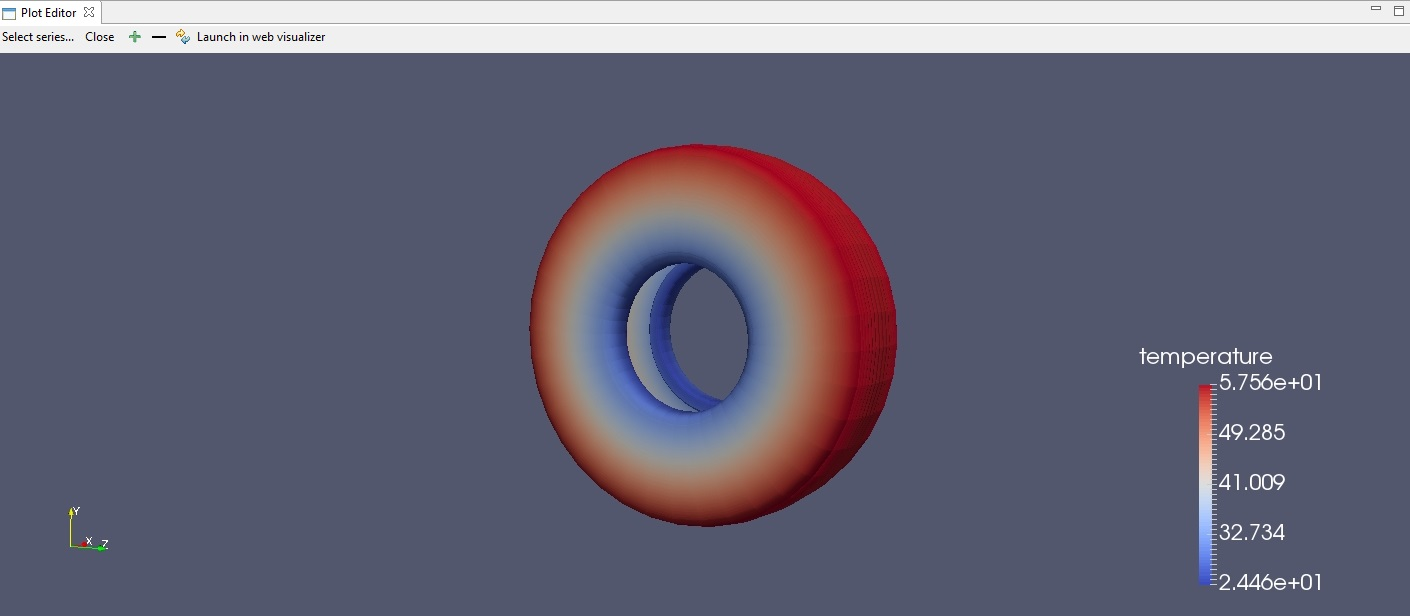
\includegraphics[width=12cm]{images/ParaViewPlotEditor}
\end{center}

Press the "Open in Web Visualizer" button in the top left to launch the web visualizer server and automatically open an internal web browser to view it.

\subsection{Using the Visualizer}

In order to load a data file, click the Show File List button as seen below.

\begin{center}
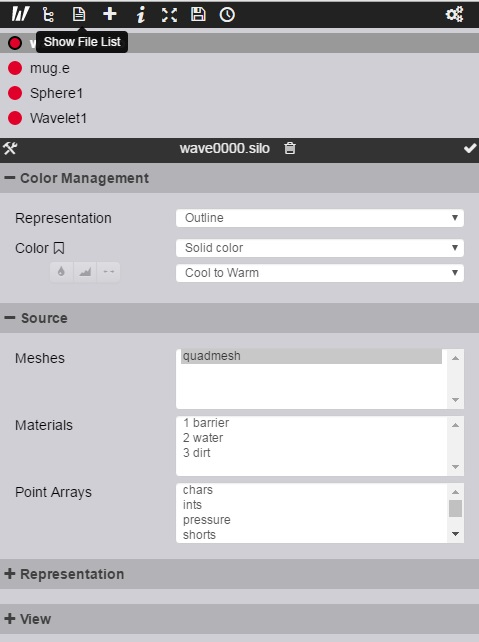
\includegraphics[width=12cm]{images/ParaViewVisualizer}
\end{center}

This will place the contents of the data directory into the side bar. For sessions, the data directory will be your ICE workspace. For a remote connection, this will be the folder containing the remote file you are visualizing. You may then double click on a file to load it into the model. 

You can click and drag the mouse to rotate the camera and right click followed
by dragging up or down to zoom. A full description of the visualizer's features
is beyond the scope of this tutorial, but see the official documentation
\href{http://www.paraview.org/ParaView3/Doc/Nightly/www/js-doc/index.html#!/guide/web_visualizer}{here}.